%%%%%%%%%%%%%%%%%%%%%%%%%%%%%%%%%%%%%%%%%%%%%%
%                insertmeeting
% 1) Title (something creative & funny?)
% 2) Date (MM/DD/YYYY)
% 3) Location (ex. Hagerty High School)
% 4) People/Committees Present 
% 5) Picture 
% 6) Start Time & Stop Time (ex. 12:30AM to 4:30PM)
%%%%%%%%%%%%%%%%%%%%%%%%%%%%%%%%%%%%%%%%%%%%%%
\insertmeeting 
	{Incredible Intakes} 
	{11/18/21}
	{Hagerty High School}
	{Clayton, Nathan, Ritam}
	{Images/RobotPics/robot.jpg}
	{2:30 - 4:30}
	
\hhscommittee{Hardware}
\noindent\hfil\rule{\textwidth}{.4pt}\hfil
\subsubsection*{Goals}
\begin{itemize}
    \item started creating CAD for intake
    \item Used more variables in case of future changes
 

\end{itemize} 

\noindent\hfil\rule{\textwidth}{.4pt}\hfil

\subsubsection*{Accomplishments}
Taking inspiration from our sketches we made at the last meeting, we started creating our new roller intake design in Onshape. Knowing there would likely be future changes to the design, we focused on creating variables for any critical dimensions that would allow us to easily change almost any part of the design without having to fix errors. By the time we finished CADing, our final variable list ended up having quite a lot of variables, all of which are connected to different parts or dimensions of the model (Figure \ref{fig:pic1}). We started creating the geometry by adding the sides that would hold bearings for the coaxial arm and by creating the back stop for the block. To connect all of this to the robot, we wanted to switch our arm to a lighter and more efficient material like carbon fiber or graphite. Because we were unsure what size this pole would be, we created a variable for it that will allow us to seamlessly change it later. With this in mind, we created a pole attachment point where the pole and intake will connect (Figure \ref{fig:pic2}).  We then added a bottom plate that will screw into a fiberglass plate which the block will slide onto and be supported by. Around this point, we realized a flaw with our design. The robot's backstop plate hits the top of the arm when we lower the arm all the way back. This is a problem because with our original plan, there would be a belt running across the top of the arm connecting the servo to the coaxial arm. To counteract this, we decided to run the belt along the bottom of the intake, then redirect it up to the coaxial arm with a pulley at the bottom of the intake. We created a hole for the pulley in CAD and added some ribs for support (Figure \ref{fig:pic3}). To complete this design, we added fillets and pocketing holes to make the design lighter and stronger (Figure \ref{fig:pic4}). Finally we put the parts together in an assembly (Figure \ref{fig:pic5}). Although the design is incomplete, we feel that it is quite promising and thanks to our generous use of variables, should be adaptable to any future changes.

 

\begin{figure}[ht]
\centering
\begin{minipage}[b]{.48\textwidth}
  \centering
  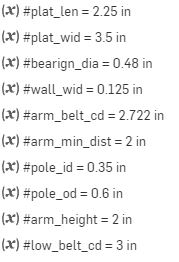
\includegraphics[width=0.95\textwidth]{Meetings/November/11-18-21/11-18-21_CAD_Figure1 - Nathan Forrer.JPG}
  \caption{A variable list for future usee}
  \label{fig:pic1}
\end{minipage}%
\hfill%
\begin{minipage}[b]{.48\textwidth}
  \centering
  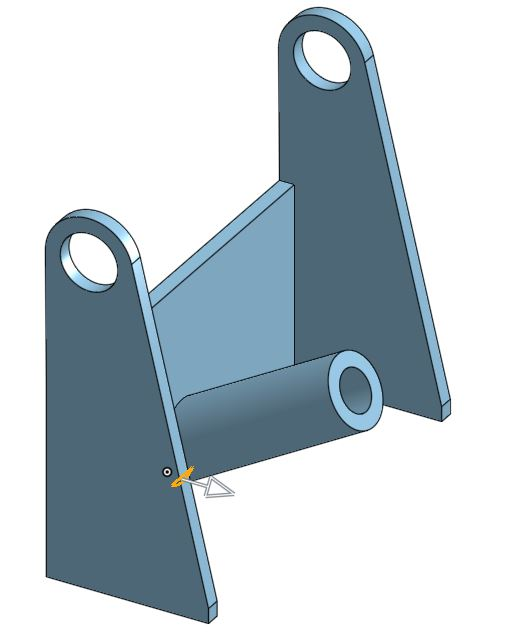
\includegraphics[width=0.95\textwidth]{Meetings/November/11-18-21/11-18-21_CAD_Figure2 - Nathan Forrer.JPG}
  \caption{CAD for the pole attachment point}
  \label{fig:pic2}
\end{minipage}
\end{figure}

\begin{figure}[ht]
\centering
\begin{minipage}[b]{.48\textwidth}
  \centering
  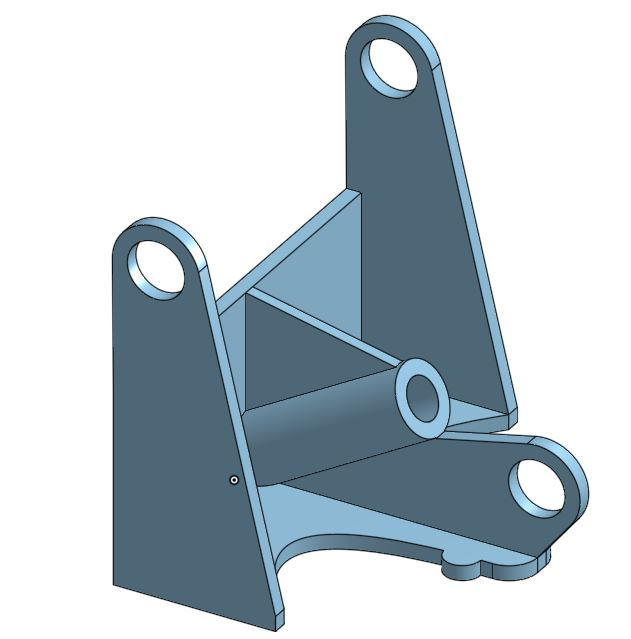
\includegraphics[width=0.95\textwidth]{Meetings/November/11-18-21/11-18-21_CAD_Figure3 - Nathan Forrer.JPG}
  \caption{Adding a pulley mounting point}
  \label{fig:pic3}
\end{minipage}%
\hfill%
\begin{minipage}[b]{.48\textwidth}
  \centering
  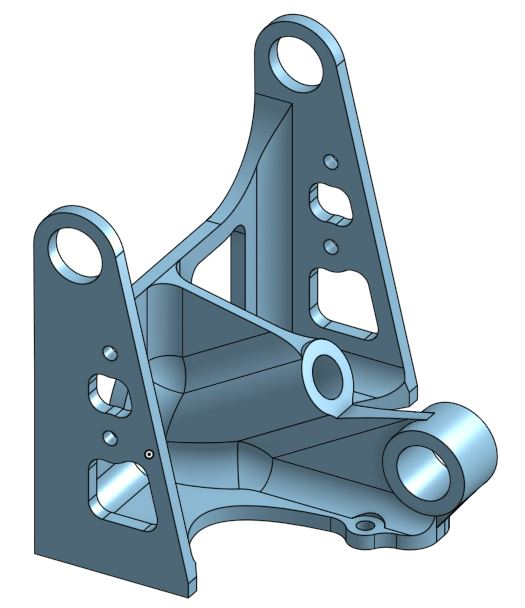
\includegraphics[width=0.95\textwidth]{Meetings/November/11-18-21/11-18-21_CAD_Figure4 - Nathan Forrer.JPG}
  \caption{Completing the design}
  \label{fig:pic4}
\end{minipage}
\end{figure}


\begin{figure}[htp]
\centering
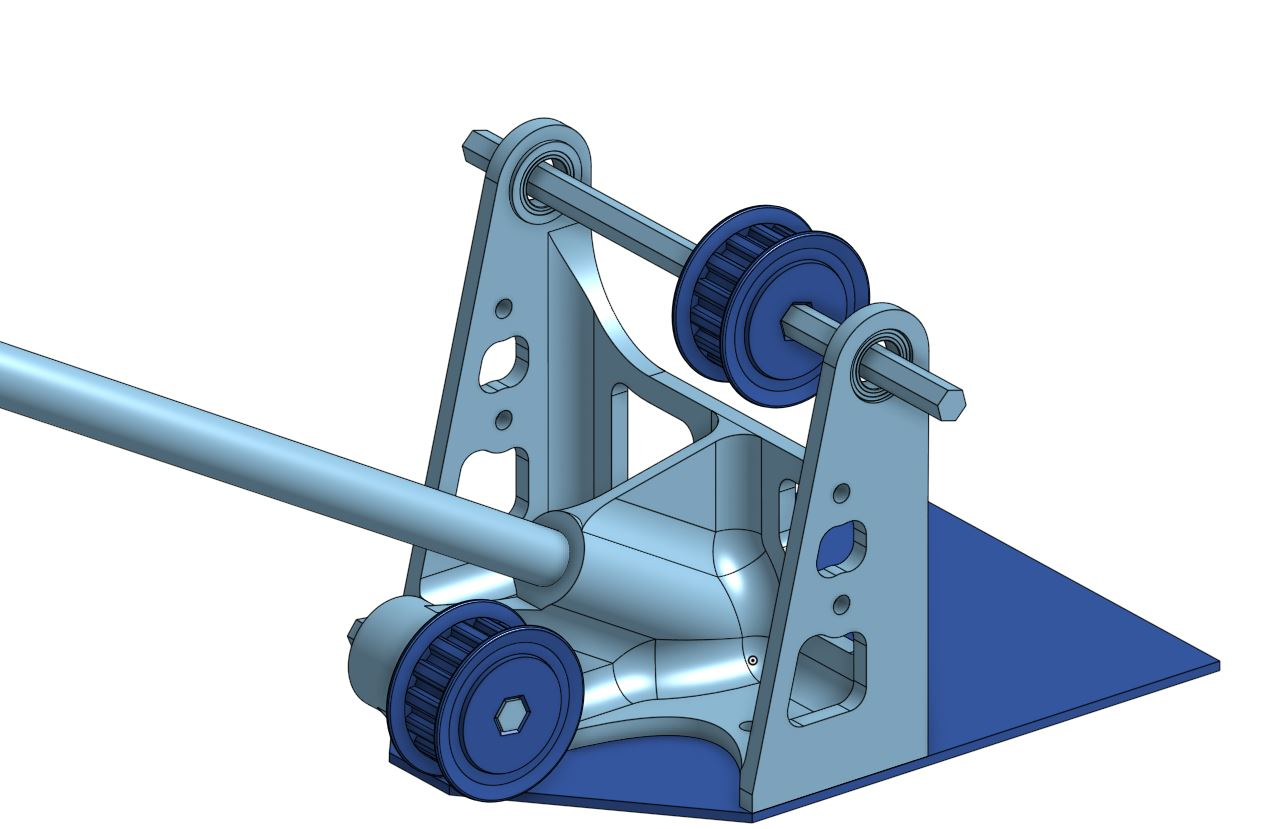
\includegraphics[width=0.95\textwidth, angle=0]{Meetings/November/11-18-21/11-18-21_CAD_Figure5.JPG}
\caption{The completed assembly}
\label{fig:pic5}
\end{figure}


\whatsnext{
\begin{itemize}
    \item Complete the CAD for the intake
\end{itemize} 
}

